\chapter{Descarga e instalación del proyecto}
\label{Appendix:Key1}

El código desarrollado durante la realización de este trabajo se encuentra disponible en el
repositorio: \url{https://github.com/tronxi/real-time-tracking-system}

Todos los componentes desarrollados para la plataforma de visualización se encuentran dockerizados, por tanto la única herramienta necesaria para desplegar la plataforma es Docker.

El primer paso es clonar el repositorio y acceder a la carpeta docker-compose:

\begin{figure}[H]
    \centering
    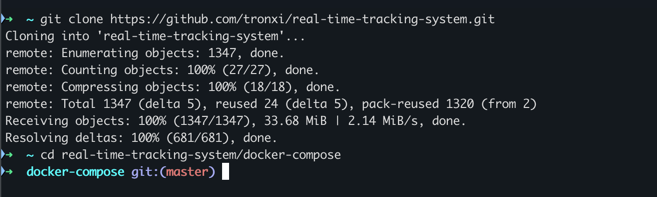
\includegraphics[width=1\textwidth]{Imagenes/Bitmap/clone}
    \caption{Clonado del repositorio}
    \label{fig:clone}
\end{figure}

A continuación, se debe ejecutar el siguiente comando para construir y lanzar todos los servicios:

\begin{verbatim}
docker compose up -d --build
\end{verbatim}

Este comando creará los contenedores necesarios utilizando los \texttt{Dockerfile} definidos en cada componente.
para verificar que se han desplegado correctamente, puede utilizarse:

\begin{verbatim}
docker ps
\end{verbatim}

\begin{figure}[H]
    \centering
    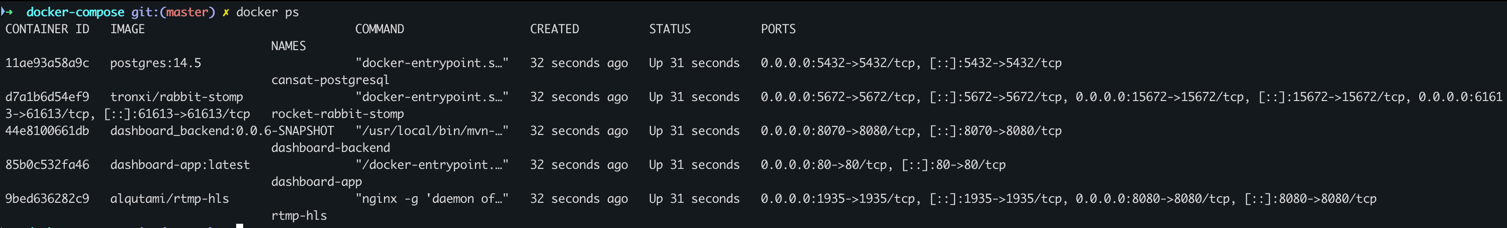
\includegraphics[width=1\textwidth]{Imagenes/Bitmap/ps}
    \caption{Ejecucción del comando docker ps}
    \label{fig:ps}
\end{figure}

Como podemos ver en la salida del comando tendremos los servicios levantados en los siguientes puertos:
\begin{itemize}
    \item \textbf{Interfaz web:} \url{http://localhost}
    \item \textbf{Backend:} \url{http://localhost:8070}
    \item \textbf{PostgreSQL:} \texttt{localhost:5432}
    \item \textbf{RabbitMQ:} \url{http://localhost:15672}
    \item \textbf{Servidor RTMP:} \url{http://localhost:8080}
\end{itemize}

Las credenciales y contraseñas necesarias para los distintos servicios están definidas como variables de entorno en el fichero \texttt{.env}, ubicado en la carpeta \texttt{docker-compose/}. Estas pueden modificarse para adaptarlas a las necesidades de cada proyecto.

\begin{figure}[H]
    \centering
    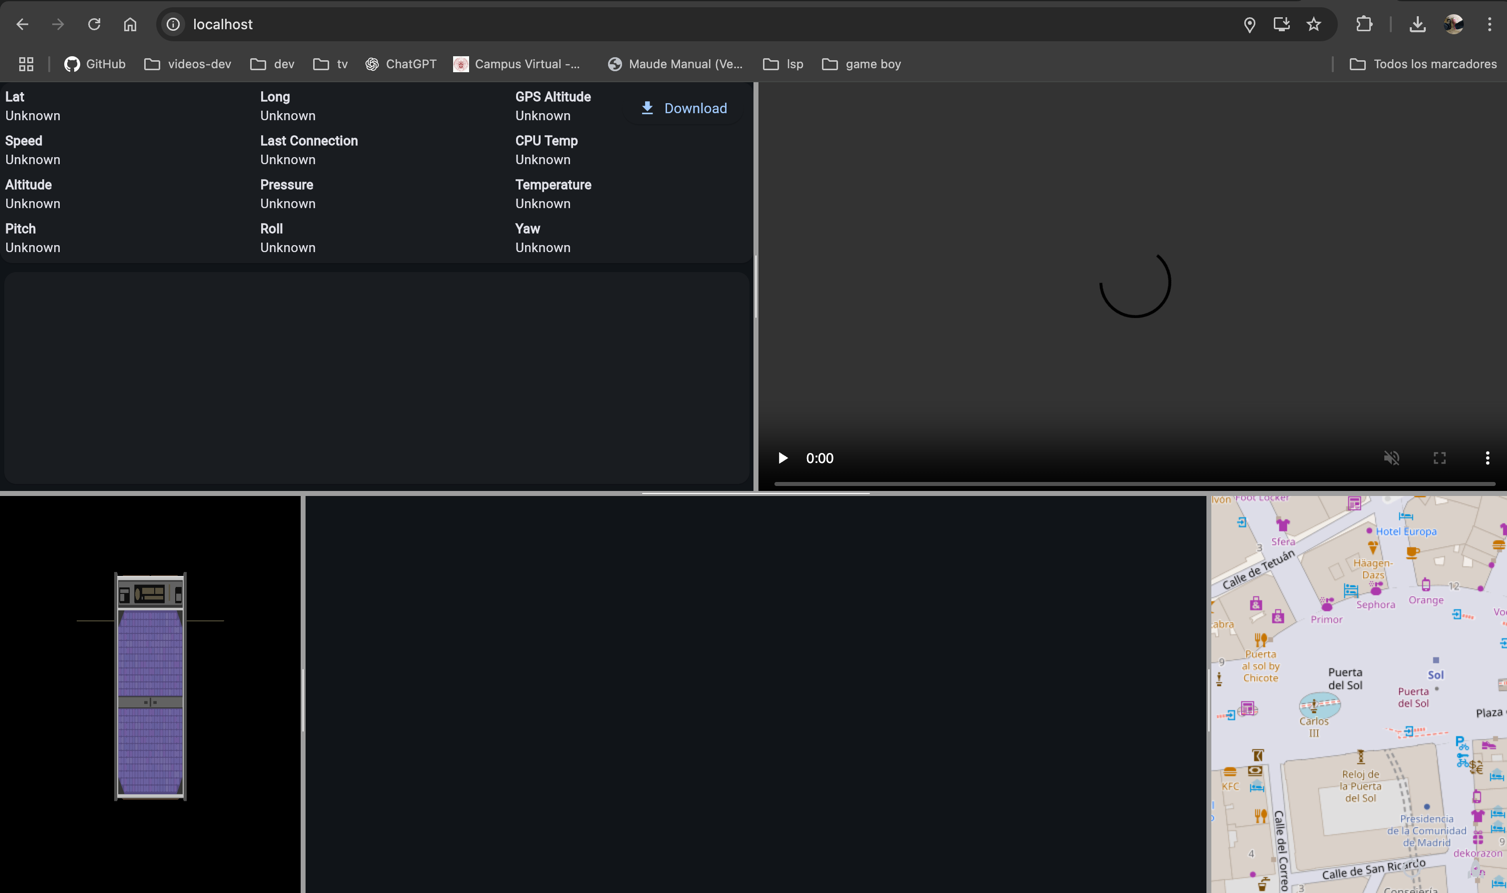
\includegraphics[width=1\textwidth]{Imagenes/Bitmap/interfaz_local}
    \caption{Interfaz Web corriendo en el puerto 80}
    \label{fig:interfaz_local}
\end{figure}

\begin{figure}[H]
    \centering
    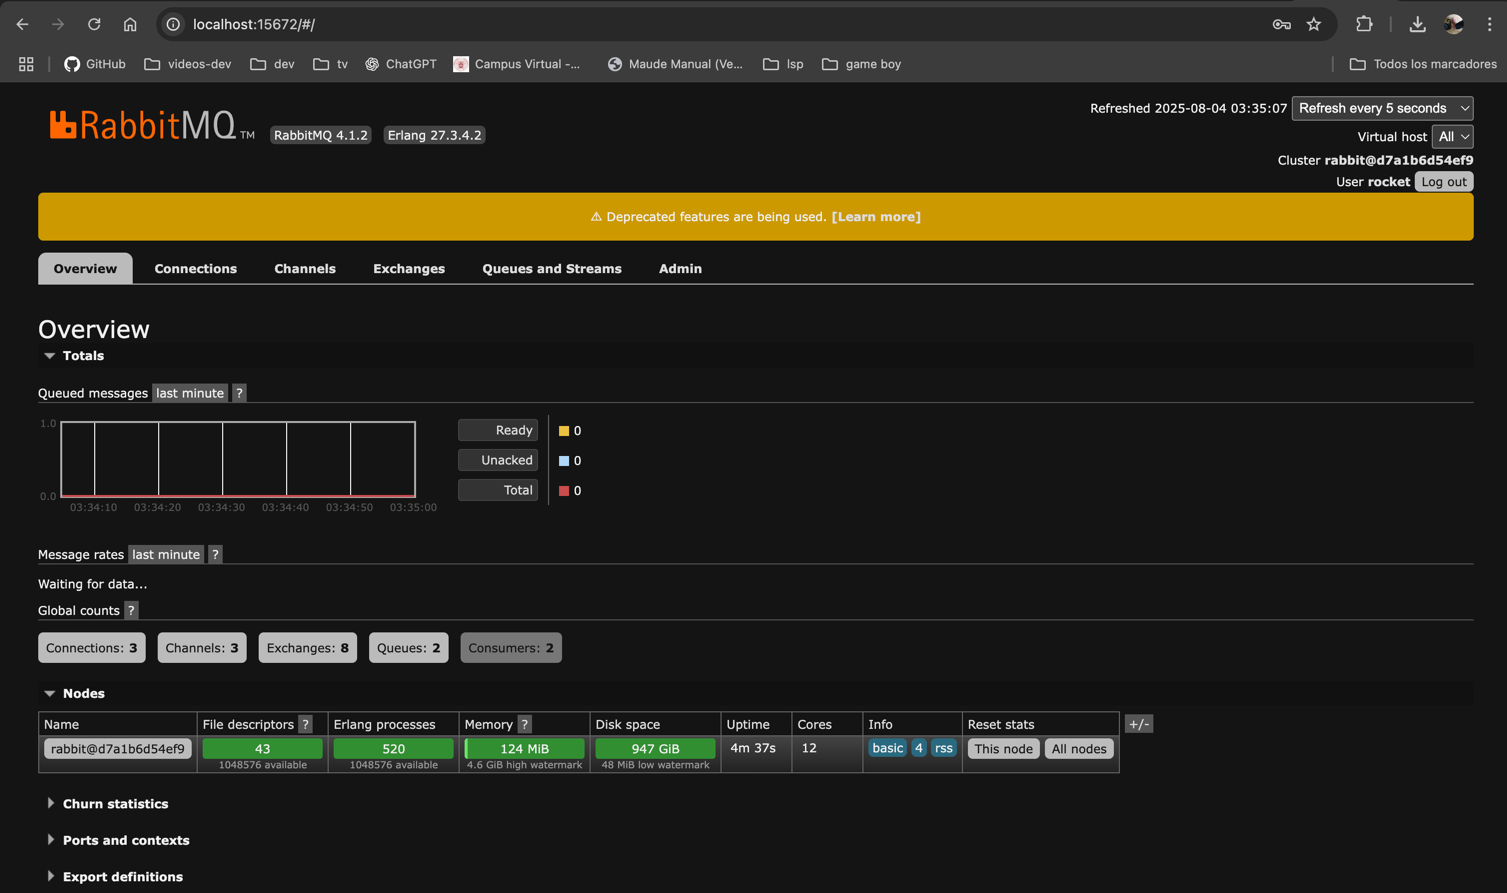
\includegraphics[width=1\textwidth]{Imagenes/Bitmap/interfaz_rabbit}
    \caption{Interfaz RabbitMQ corriendo en el puerto 15672}
    \label{fig:interfaz_rabbit}
\end{figure}
